\chapter{Results}

\section{Preparation}
\begin{figure}[h]
    \centering
    \begin{subfigure}{0.25\textwidth}
        \includegraphics[width = \textwidth]{Plots/Fe.png}
        \caption{}
        \label{fig:leed_Fe}
    \end{subfigure}
    \hfill
    \begin{subfigure}{0.25\textwidth}
        \includegraphics[width = \textwidth]{Plots/FeO.png}
        \caption{}
        \label{fig:leed_FeO}
    \end{subfigure}
    \hfill
    \begin{subfigure}{0.25\textwidth}
        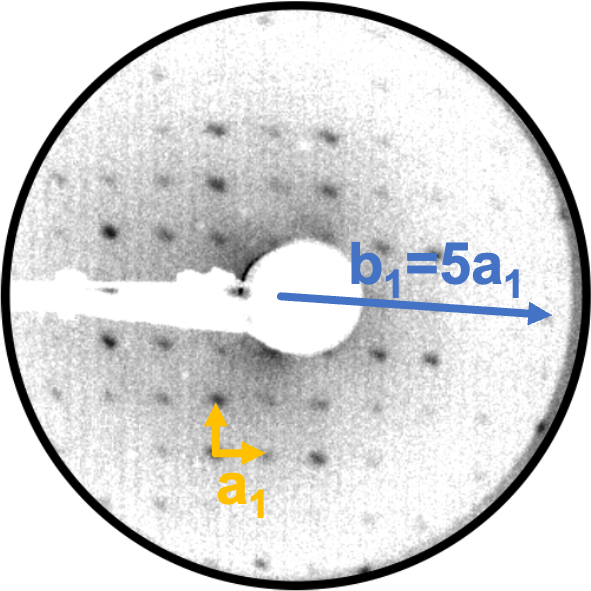
\includegraphics[width = \textwidth]{Plots/FeO_ZnTPP.png}
        \caption{}
        \label{fig:leed_FeO_ZnTPP}
    \end{subfigure}
    \caption{LEED image of the \textbf{(a)} Fe(100) surface, taken at an electron beam energy of \qty{90}{eV}, the \textbf{(b)} Fe(100)-\textit{p}(1\times1)O surface, taken at an electron beam energy of \qty{90}{eV} and \textbf{(c)} the Fe(100)-\textit{p}(1\times1)O/ZnTPP surface, taken at an electron beam energy of \qty{32}{eV}, where an ordered 1ML coverage can be deduced.}
    \label{fig:leed_1}
\end{figure}
\FloatBarrier

To confirm the quality of the Fe(100)-\textit{p}(1\times1)O surfac, a LEED image was taken before and after passivation at the same electron beam energy of \qty{90}{eV}, displayed in Figures \ref{fig:leed_Fe} and \ref{fig:leed_FeO}.
The comparison to the clean surface shows no degradation of the spot sharpness, which indicates a complete monolayer coverage without contamination.
There is also no change in spot position, so that a (1\times1) reconstruction of oxygen atoms can be confirmed.
As can be seen in \autoref{fig:leed_FeO_ZnTPP} the ZnTPP forms a commensurate square (5\times5) super-lattice, which shows a certain interaction with the substrate, not strong enough to form islands like seen on a clean Fe(100) surface \cite*{bussetti_structure_2016}, but present enough to still interact with the substrate and self-assembly in an ordered way.
The reciprocal lattice constant of the underlying substrate $a_1$ is five times the reciprocal lattice constant of the reconstruction $b_1$, meaning that the ZnTPP molecules are apart $14,25\,$\r{A}, five times the Fe lattice constant $2,85\,$\r{A} \cite*{davey_precision_1925}.

\begin{figure}[h]
    \centering
    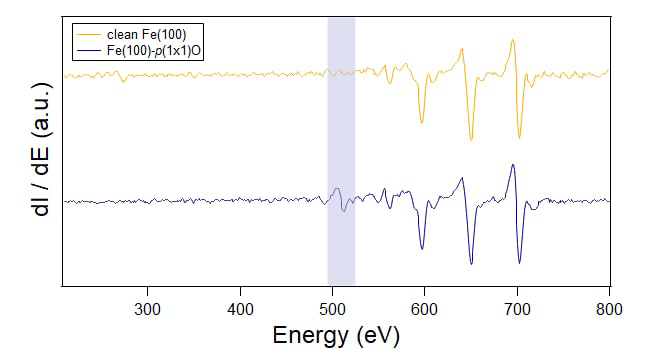
\includegraphics[width = 0.7\textwidth]{Plots/Auger.png}
    \caption{The derived intensity of the Auger spectra after cleaning the Fe(100) surface (top) and after passivation (bottom). The oxygen peak is located at \qty{503}{eV} and highlighted in the graph.}
    \label{fig:auger_FeO}
\end{figure}
\FloatBarrier
Comparing the Auger spectra of the clean and passivated Fe(100) surface also shows a significant increase in the peak at \qty{503}{eV} belonging to oxygen.
From a chemical composition point of view this poses as another confirmation, that the Fe(100) surface was successfully passivated.

For the clean Cu(100) substrate, as expected, a square lattice can be seen in \autoref{fig:leed_Cu}.
After deposition of the ZnTPP molecules on the surface, a complex LEED pattern due to several domains is visible in \autoref{fig:leed_Cu_ZnTPP}.
There could not be found a commensurate super-lattice, which would recreate this pattern, but the sharp spots clearly show an ordered assembly of the molecules on the Cu(100) substrate and indictae a 1ML coverage.
\begin{figure}[h]
    \centering
    \begin{subfigure}{0.49\textwidth}
        \centering
        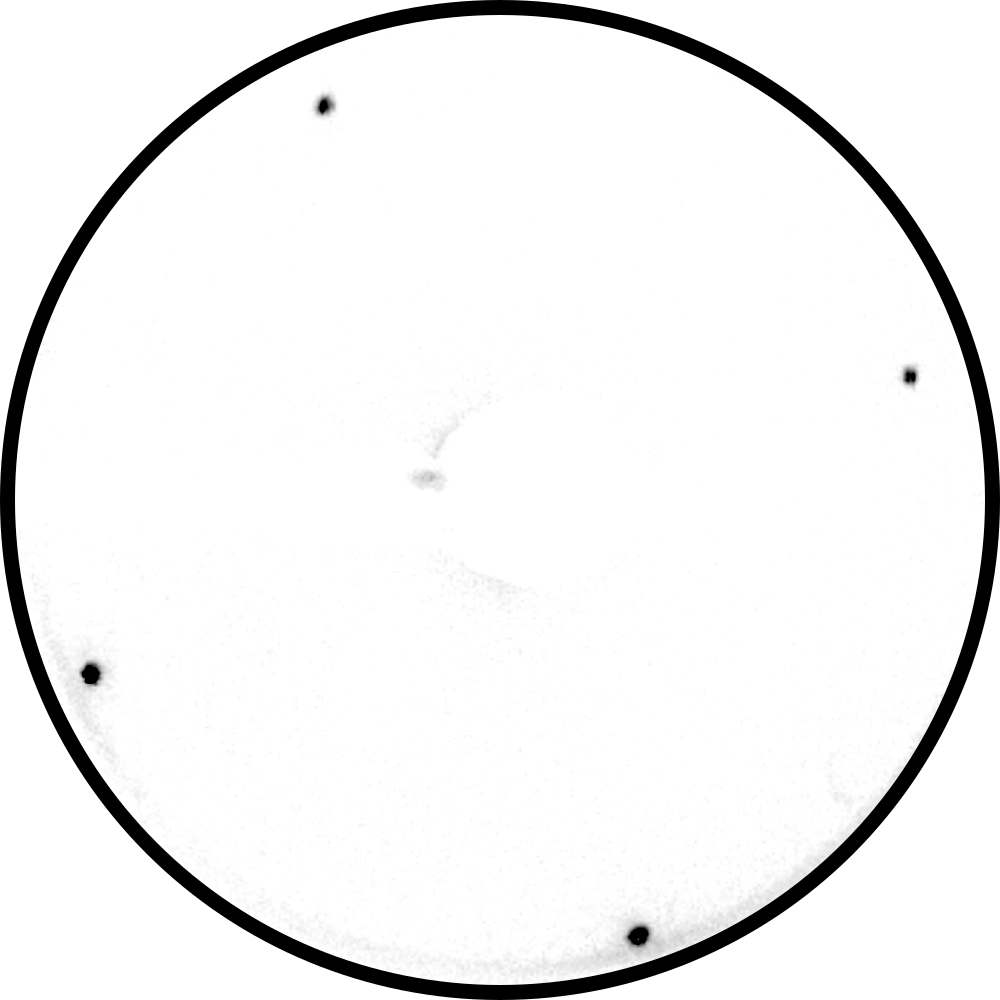
\includegraphics[width = 0.5\textwidth]{Plots/Cu.png}
        \caption{}
        \label{fig:leed_Cu}
    \end{subfigure}
    \hfill
    \begin{subfigure}{0.49\textwidth}
        \centering
        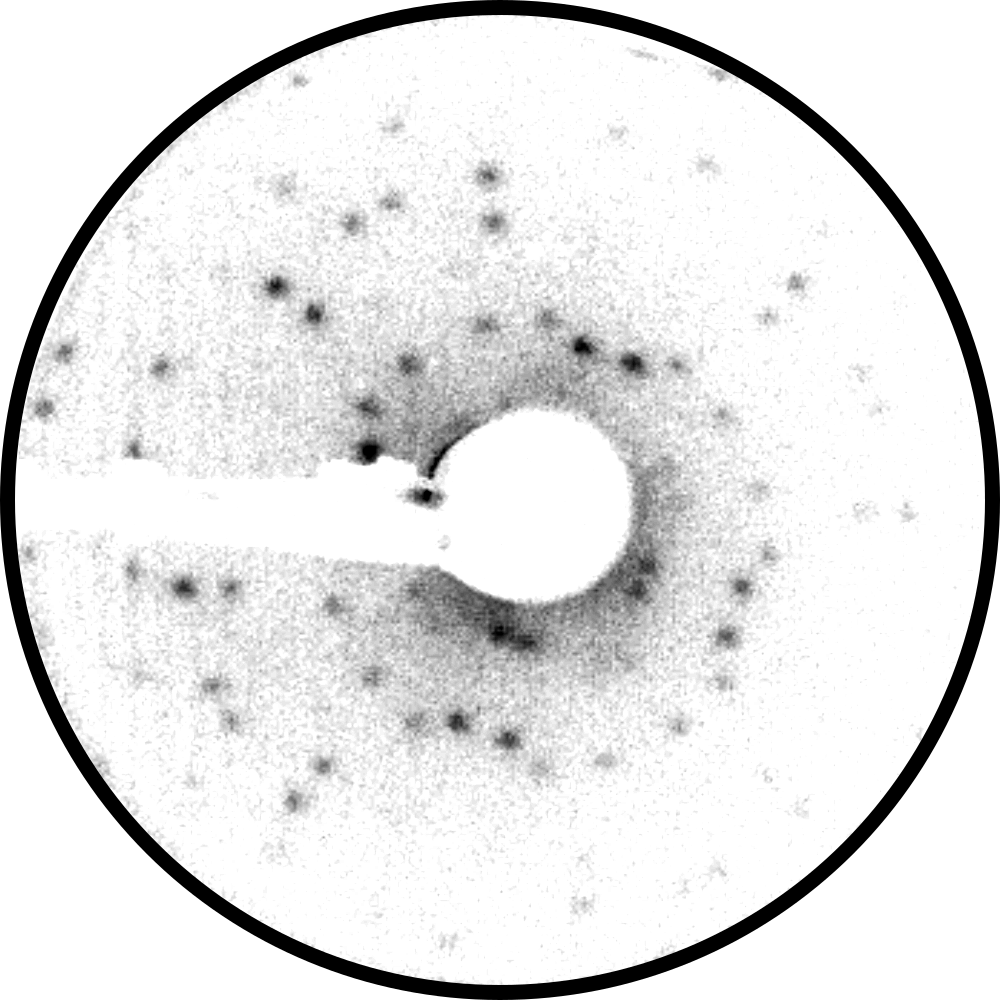
\includegraphics[width = 0.5\textwidth]{Plots/Cu_ZnTPP.png}
        \caption{}
        \label{fig:leed_Cu_ZnTPP}
    \end{subfigure}
    \caption{LEED image of the \textbf{(a)} Cu(100) surface, taken at an electron beam energy of \qty{44}{eV} and \textbf{(b)} the Cu(100)/ZnTPP surface, taken at an electron beam energy of \qty{32}{eV}.}
    \label{fig:leed_2}
\end{figure}
\FloatBarrier

\newpage
\section{Electronic structure characterization}
\begin{figure}[h]
    \centering
    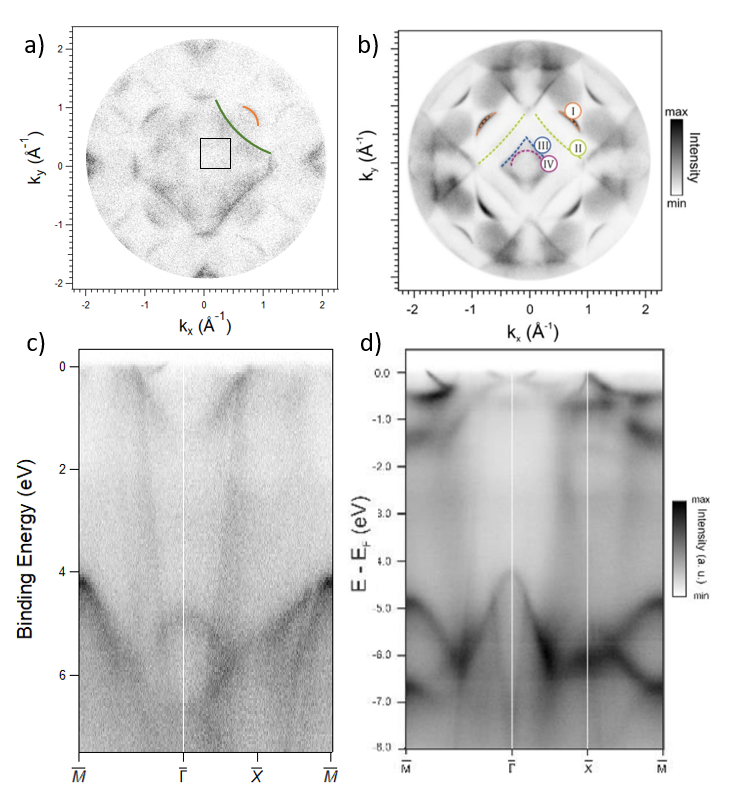
\includegraphics[width = 0.7\textwidth]{Plots/bandstructure.png}
    \caption{Momentum maps at the fermi level (top) and the bandstructure for the Fe(100)-\textit{p}(1\times1)O surface along the $\overline{\text{M}}$-$\overline{\Upgamma}$-$\overline{\text{X}}$-$\overline{\text{M}}$ line (bottom). The data displayed in \textbf{(a)} and \textbf{(c)} was measured with the He lamp, \textbf{(b)} and \textbf{(d)} were taken from \cite*{janas_enhancing_2022}, where the data was aquired at a synchrotron.}
    \label{fig:bandstructure}
\end{figure}
\FloatBarrier
As reported from Janas et al. \cite*{janas_enhancing_2022} and displayed in \autoref{fig:bandstructure}b the momentum map for the passivated Fe(100) surface at the fermi level shows distinct features numbered I to IV.
In our data (\autoref{fig:bandstructure}a) we can verify the features I and II, highlighted by lines drawn in the upper right quarter of the map.
The features III and IV around the $\overline{\Upgamma}$ point (black square) can not be confirmed in our data.
It should be noted, that the momentum map of Janas et al. \cite*{janas_enhancing_2022} was taken at a photon energy of \qty{64}{eV}.
This corresponds to a sphere cutting the 3D bulk brillouin zone at a different energy value, meaning that features changing 
with the photon energy are related to the bulk crystal.
The bandstructure (\autoref{fig:bandstructure}d) taken at a lower photon energy of \qty{30}{eV}, comparable to the He lamp energy used to aquire our data, shows a lower intensity for the features near the $\overline{\Upgamma}$ point at the fermi level,
contrary to the measurements at higher photon energies (see \autoref{fig:bandstructure}b and supplementary information of \cite*{janas_enhancing_2022}). 
Upholding the before stated claim, these states can therefore be ascribed to the bulk crystal.

In our bandstructure displayed in \autoref{fig:bandstructure}c one can clearly see the oxygen 2\textit{p} bands, even though they are shifted in energy in comparison to \autoref{fig:bandstructure}d. Around the $\overline{\Upgamma}$ point the bands lie \qty{1}{eV} lower and near the $\overline{\text{M}}$ point \qty{1}{eV} higher in binding energy.





\begin{figure}[h]
    \centering
    \begin{subfigure}{0.49\textwidth}
        \centering
        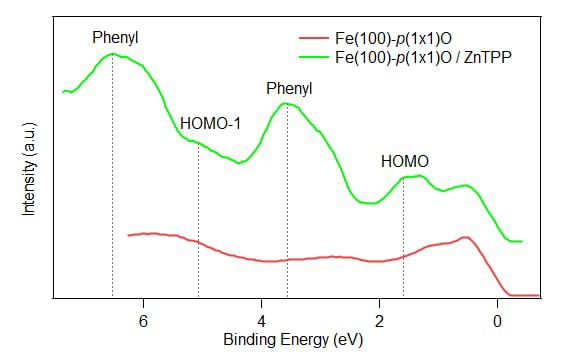
\includegraphics[width = \textwidth]{Plots/integrated_spectrum_Fe.png}
        \caption{}
        \label{fig:ups_spectrum}
    \end{subfigure}
    \hfill
    \begin{subfigure}{0.49\textwidth}
        \centering
        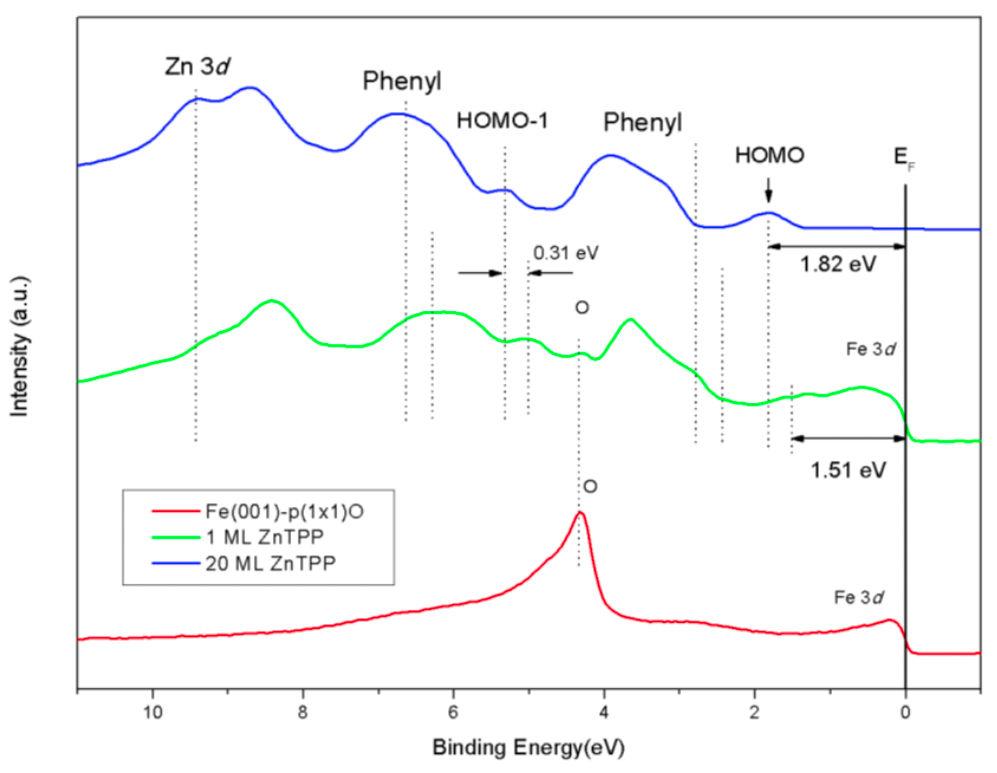
\includegraphics[width = \textwidth]{Plots/integrated_spectrum_Fe_lit.png}
        \caption{}
        \label{fig:ups_spectrum_lit}
    \end{subfigure}
    \caption{\textbf{(a)} The UPS spectrum measured for the Fe(100)-\textit{p}(1\times1)O substrate and 1ML adsorbed ZnTPP at a photon energy of $h\nu = \qty{29.8}{eV}$ with the HHG. \\\textbf{(b)} The UPS spectrum for the Fe(100)-\textit{p}(1\times1)O system, as well as 1ML and 20 ML coverage, taken from \cite*{tesi}.}
    \label{fig:ups}
\end{figure}
\FloatBarrier
Using the UPS spectrum \autoref{fig:ups_spectrum_lit} taken from literature \cite*{tesi}, the main features of our measured spectrum in \autoref{fig:ups_spectrum} could be identified.
A clear difference in the spectra of the Fe(100)-\textit{p}(1\times1)O substrate can be seen in the oxygen peak. In \autoref{fig:ups_spectrum_lit} it is located at a binding energy of \qty{4.36}{eV} and quite narrow, considerably exceeding the valence band in height. 
On the other hand, in our data the oxygen forms a broad feature starting at a binding energy of around \qty{4.5}{eV} and a maximum at around \qty{6}{eV}.
Nevertheless in \autoref{fig:bandstructure}c the oxygen 2\textit{p} bands are clearly visibly.
The green line corresponds to the 1ML ZnTPP coverage and here the main electronic peaks can be matched to the ones from the literature.
The HOMO is measured to be at \qty{1.6}{eV} binding energy and the HOMO-1 at approximately \qty{5.1}{eV} binding energy, which coincides well with the values in \autoref{fig:ups_spectrum_lit}.
The Fe $3d$ states near the fermi level can still be observed and do not overlap with any molecular peaks.

The UPS spectrum of Cu(100)/ZnTPP shows no distinctive molecular peaks at the 1ML molecule coverage in the observed energy range, therefore no relevant information could be gained from it.

\begin{figure}[h]
    \centering
    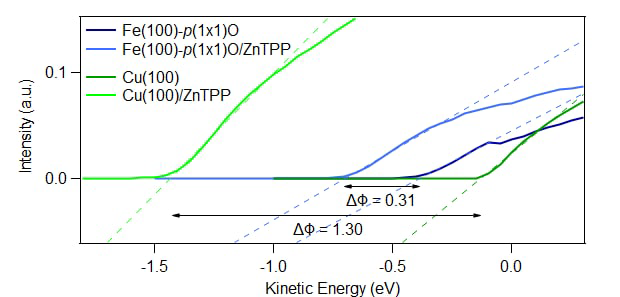
\includegraphics[width = 0.7\textwidth]{Plots/WF.png}
    \caption{Measured angle integrated spectrum at low kinetic energies and determined work function differences of both Fe(100)-\textit{p}(1\times1)O and Cu(100) substrates in relation to the respective system with a 1ML ZnTPP coverage.}
    \label{fig:wf}
\end{figure}


For both systems a reduction of the work function could be determined as shown in \autoref{fig:wf} by extrapolating the onset intersection with the energy axis. Only the difference between the absolut work function values are relevant, because the origin of the energy axis is set by the chosen sample bias voltage.
For the Fe system there is a shift of $\Delta\Phi_{\mathrm{FeO}} = \qty{0.31}{eV}$ and for the Cu system a shift of four times the size, namely $\Delta\Phi_{\mathrm{Cu}} = \qty{1.30}{eV}$, can be observed.


The reduction of the work function can be traced back to contributions of different physical and chemical effects.
Ever-present upon adsorbtion of molecules is the push-back effect, always reducing the work function.
In case of a charge transfer between substrate and adsorbat, the work function changes, depending on the direction of the charge transfer. 

In our case we can observe a stronger interaction between the Cu(100) substrate and the ZnTPP molecules, than in the Fe system, so a greater charge transfer from the Zn metal ion to the Cu(100) surface takes place.
\FloatBarrier
